\chapter{Introduzione}
Tutti i calcolatori moderni possono essere schematizzati semplicemente tramite il cosiddetto
\textbf{modello Von Neumann} in cui abbiamo tre componenti principali: \textbf{memoria},
\textbf{processore} e canali di \textbf{I/O}.

\begin{center}
	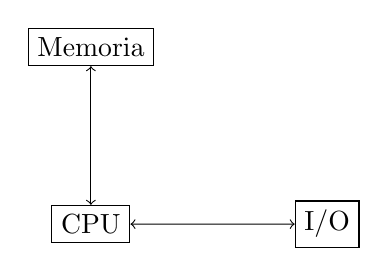
\begin{tikzpicture}[scale=1.5]
		\node[draw] (mem) at (0, 0) {Memoria};
		\node[draw] (cpu) at (0, -1.5) {CPU};
		\node[draw] (io) at (2, -1.5) {I/O};

		\draw[<->] (mem) -- (cpu);
		\draw[<->] (cpu) -- (io);
	\end{tikzpicture}
\end{center}

Come possiamo vedere dalla figura i collegamenti tra le varie entità sono bidirezionali. Il
processore (ma anche la memoria) è collegato ai canali di I/O e il collegamento che c'è tra memoria
e processore è chiamato \textbf{Von Neumann bottleneck}. Quello che accade tra memoria e processore
è, grosso modo, quello che viene descritto dal seguente pseudocodice ed è denominato ciclo di
\textbf{fetch-decode-execute}.

\begin{minted}{c}
while (true) {
	istr = M[PC]
	decode(istr)
	res = exec(istr)
	update(PC)
	writeback(res)
	interrupt_handling()
}
\end{minted}

In pratica viene estratta dalla memoria l'istruzione puntata da un \textbf{Program Counter}, la
si decodifica e la si esegue. In seguito il Program Counter viene aggiornato e i risultati vengono
consolidati nei registri della CPU oppure in memoria.

Per ognuna delle istruzioni eseguite sul canale presente tra processore e memoria vengono svolte
le seguenti operazioni
\begin{enumerate}
	\item Il processore manda un indirizzo (PC) dove andare a prendere l'istruzione.
	\item La memoria risponde con un'istruzione.
	\item Il processore esegue e durante l'esecuzione può richiedere la lettura o scrittura dalla
	      memoria.
\end{enumerate}
Questo processo avviene molto spesso e rende il traffico sul canale molto intenso creando per
l'appunto un \emph{collo di bottiglia}. Questo è dovuto alla rapida evoluzione dei processori e
alla non altrettanto rapida evoluzione della memoria, la quale ha una velocità nel fornire le
istruzioni minore della velocità che impiega il processore ad eseguirle e richiederne altre.

Per misurare le performance di un processore siamo abituati a ragionare in termini di
\textbf{cicli di clock}. Dato che, approssimativamente, possiamo dire che un ciclo di clock
corrisponde ad un'istruzione eseguita, se ad esempio abbiamo un processore a 1 GHz, questo riuscirà
ad eseguire un'istruzione in 1 nanosecondo.

\section{Architetture}
Durante il corso verrano trattate varie architetture, dalle prime progettate alle più recenti,
cercando di capire come funzionano e i loro pregi e difetti. Tra quelle che tratteremo elenchiamo
\begin{itemize}
	\item \textbf{Single cycle}: modello in cui un ciclo fetch-execute viene effettuato in un ciclo
	      di clock.
	\item \textbf{Pipeline}: modello in cui si hanno componenti distinte per le operazioni di fetch,
	      decode ed execute. In questo modo ogni componente continua a svolgere il proprio lavoro
	      parallelamente alle altre. Una volta arrivato a regime questo processore riesce a
	      eseguire un'istruzione all'inizio di ogni ciclo di clock e non alla fine (come nel
	      modello single cycle).
	\item \textbf{Superscalare}: in questo modello abbiamo, come nel modello pipeline, componenti
	      distinte che svologono compiti distinti ma invece di averne una per ogni compito, ne
	      abbiamo molteplici. Questo ci permette di eseguire più istruzioni in un singolo ciclo
	      di clock.
	\item \textbf{Multi-Core}: modello in cui si hanno più processori superscalari collegati alla
	      memoria.
\end{itemize}

Oltre a questo sono stati sviluppati anche i cosiddetti \textbf{acceleratori} come ad esempio le
GPU. Gli acceleratori sono dei processori specializzati per alcuni compiti a cui la CPU vera e
propria delega determinati calcoli tramite un canale detto \textbf{PCI Express}. Oltre alle GPU
esistono degli acceleratori per la sicurezza, i quali sono molto veloci ad eseguire calcoli
crittografici per cifrare e decifrare informazioni.

\section{Struttura}
Possiamo rappresentare il calcolatore con una serie di livelli di astrazione con una forma a stack.
Ogni livello comunica con il livello direttamente soprastante o sottostante tramite un'interfaccia
a cui i vari livelli devono conformarsi per poter comunicare.

Ogni livello possiede un grado di astrazione minore del livello soprastante e viceversa e possiamo
dire che ogni livello garantisce la ai livelli adiacenti determinati servizi.

\begin{center}
	\begin{tabular}{|c|}
		\hline
		APPLICATIVO          \\ \hline
		SISTEMA OPERATIVO    \\ \hline
		ARCHITETTURA         \\ \hline
		MICROARCHITETTURA    \\ \hline
		COMPONENTI LOGICI    \\ \hline
		DISPOSITIVI / FISICA \\ \hline
	\end{tabular}
\end{center}
